\subsection{Current Courses Page}

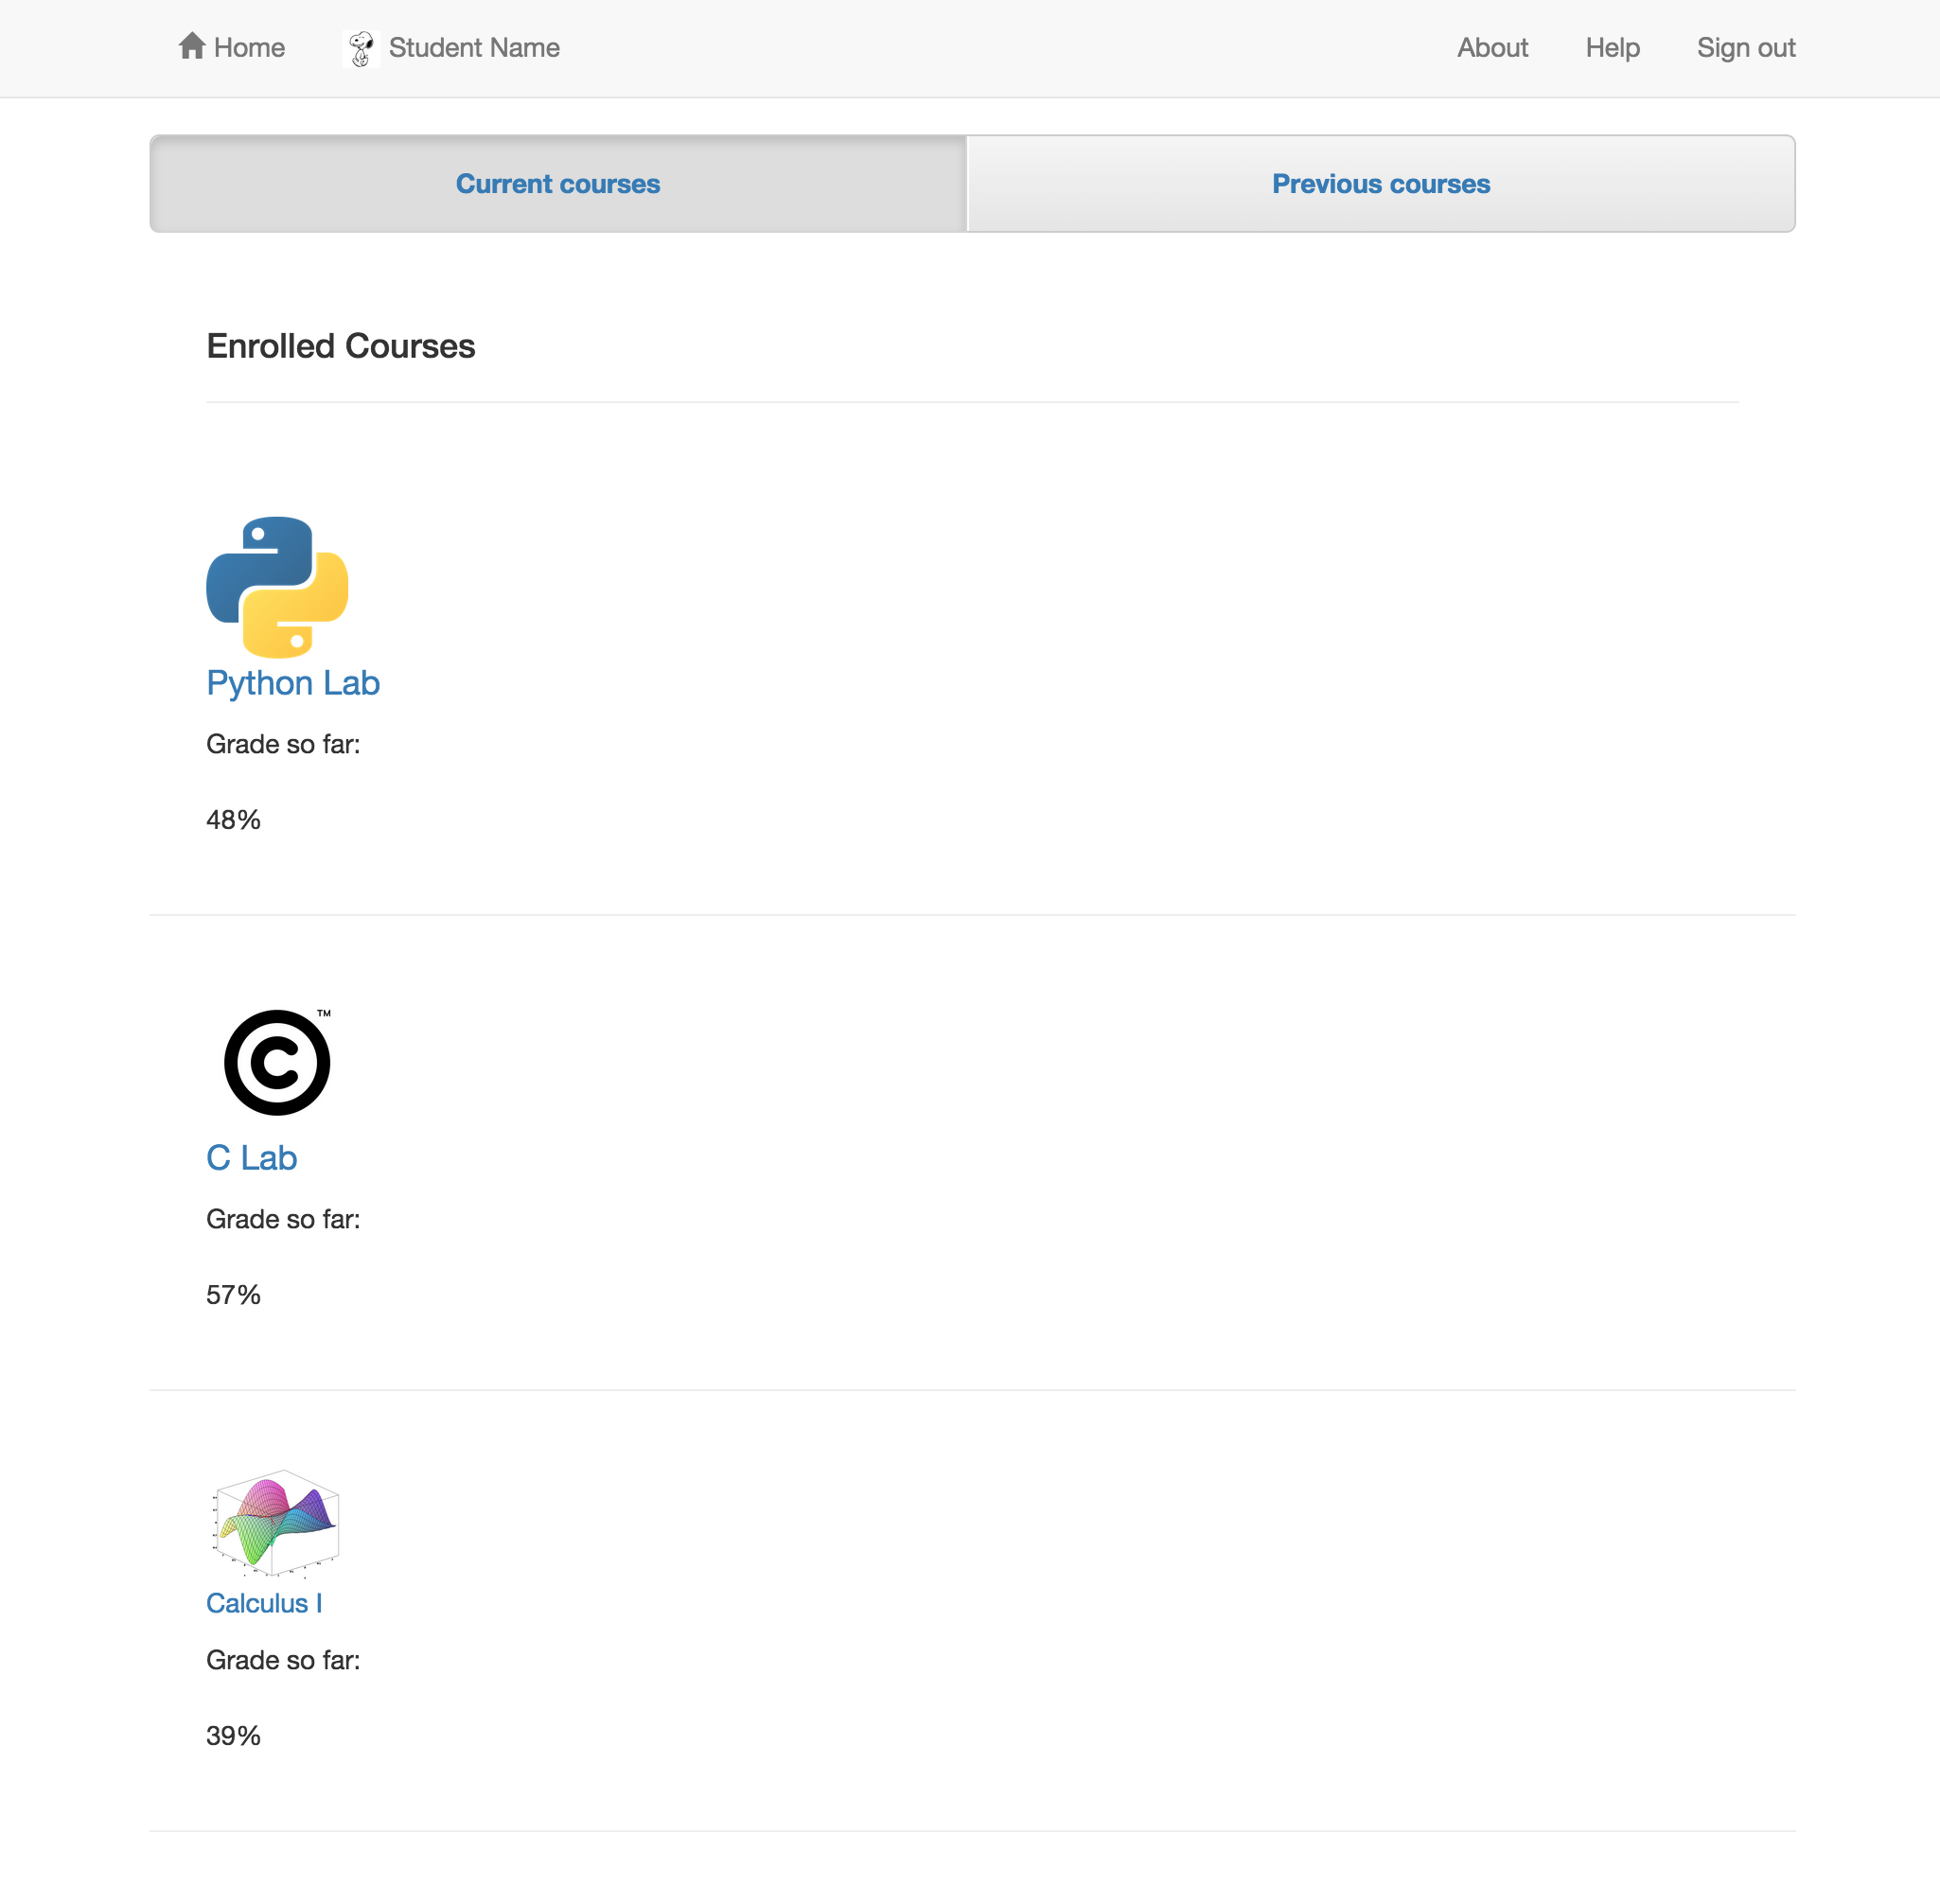
\includegraphics[width=.75\textwidth]{screenshots/CurrentCourses.png}

The current courses page features a sparse, left-justified layout in order to simplify the task of getting to the course page the user needs--minimal information beyond a grade overview, large \& attention-catching course icons, and the page navigation buttons is included. Following the rule-of-thirds by left-justifying the content helps the user process the information quicker.

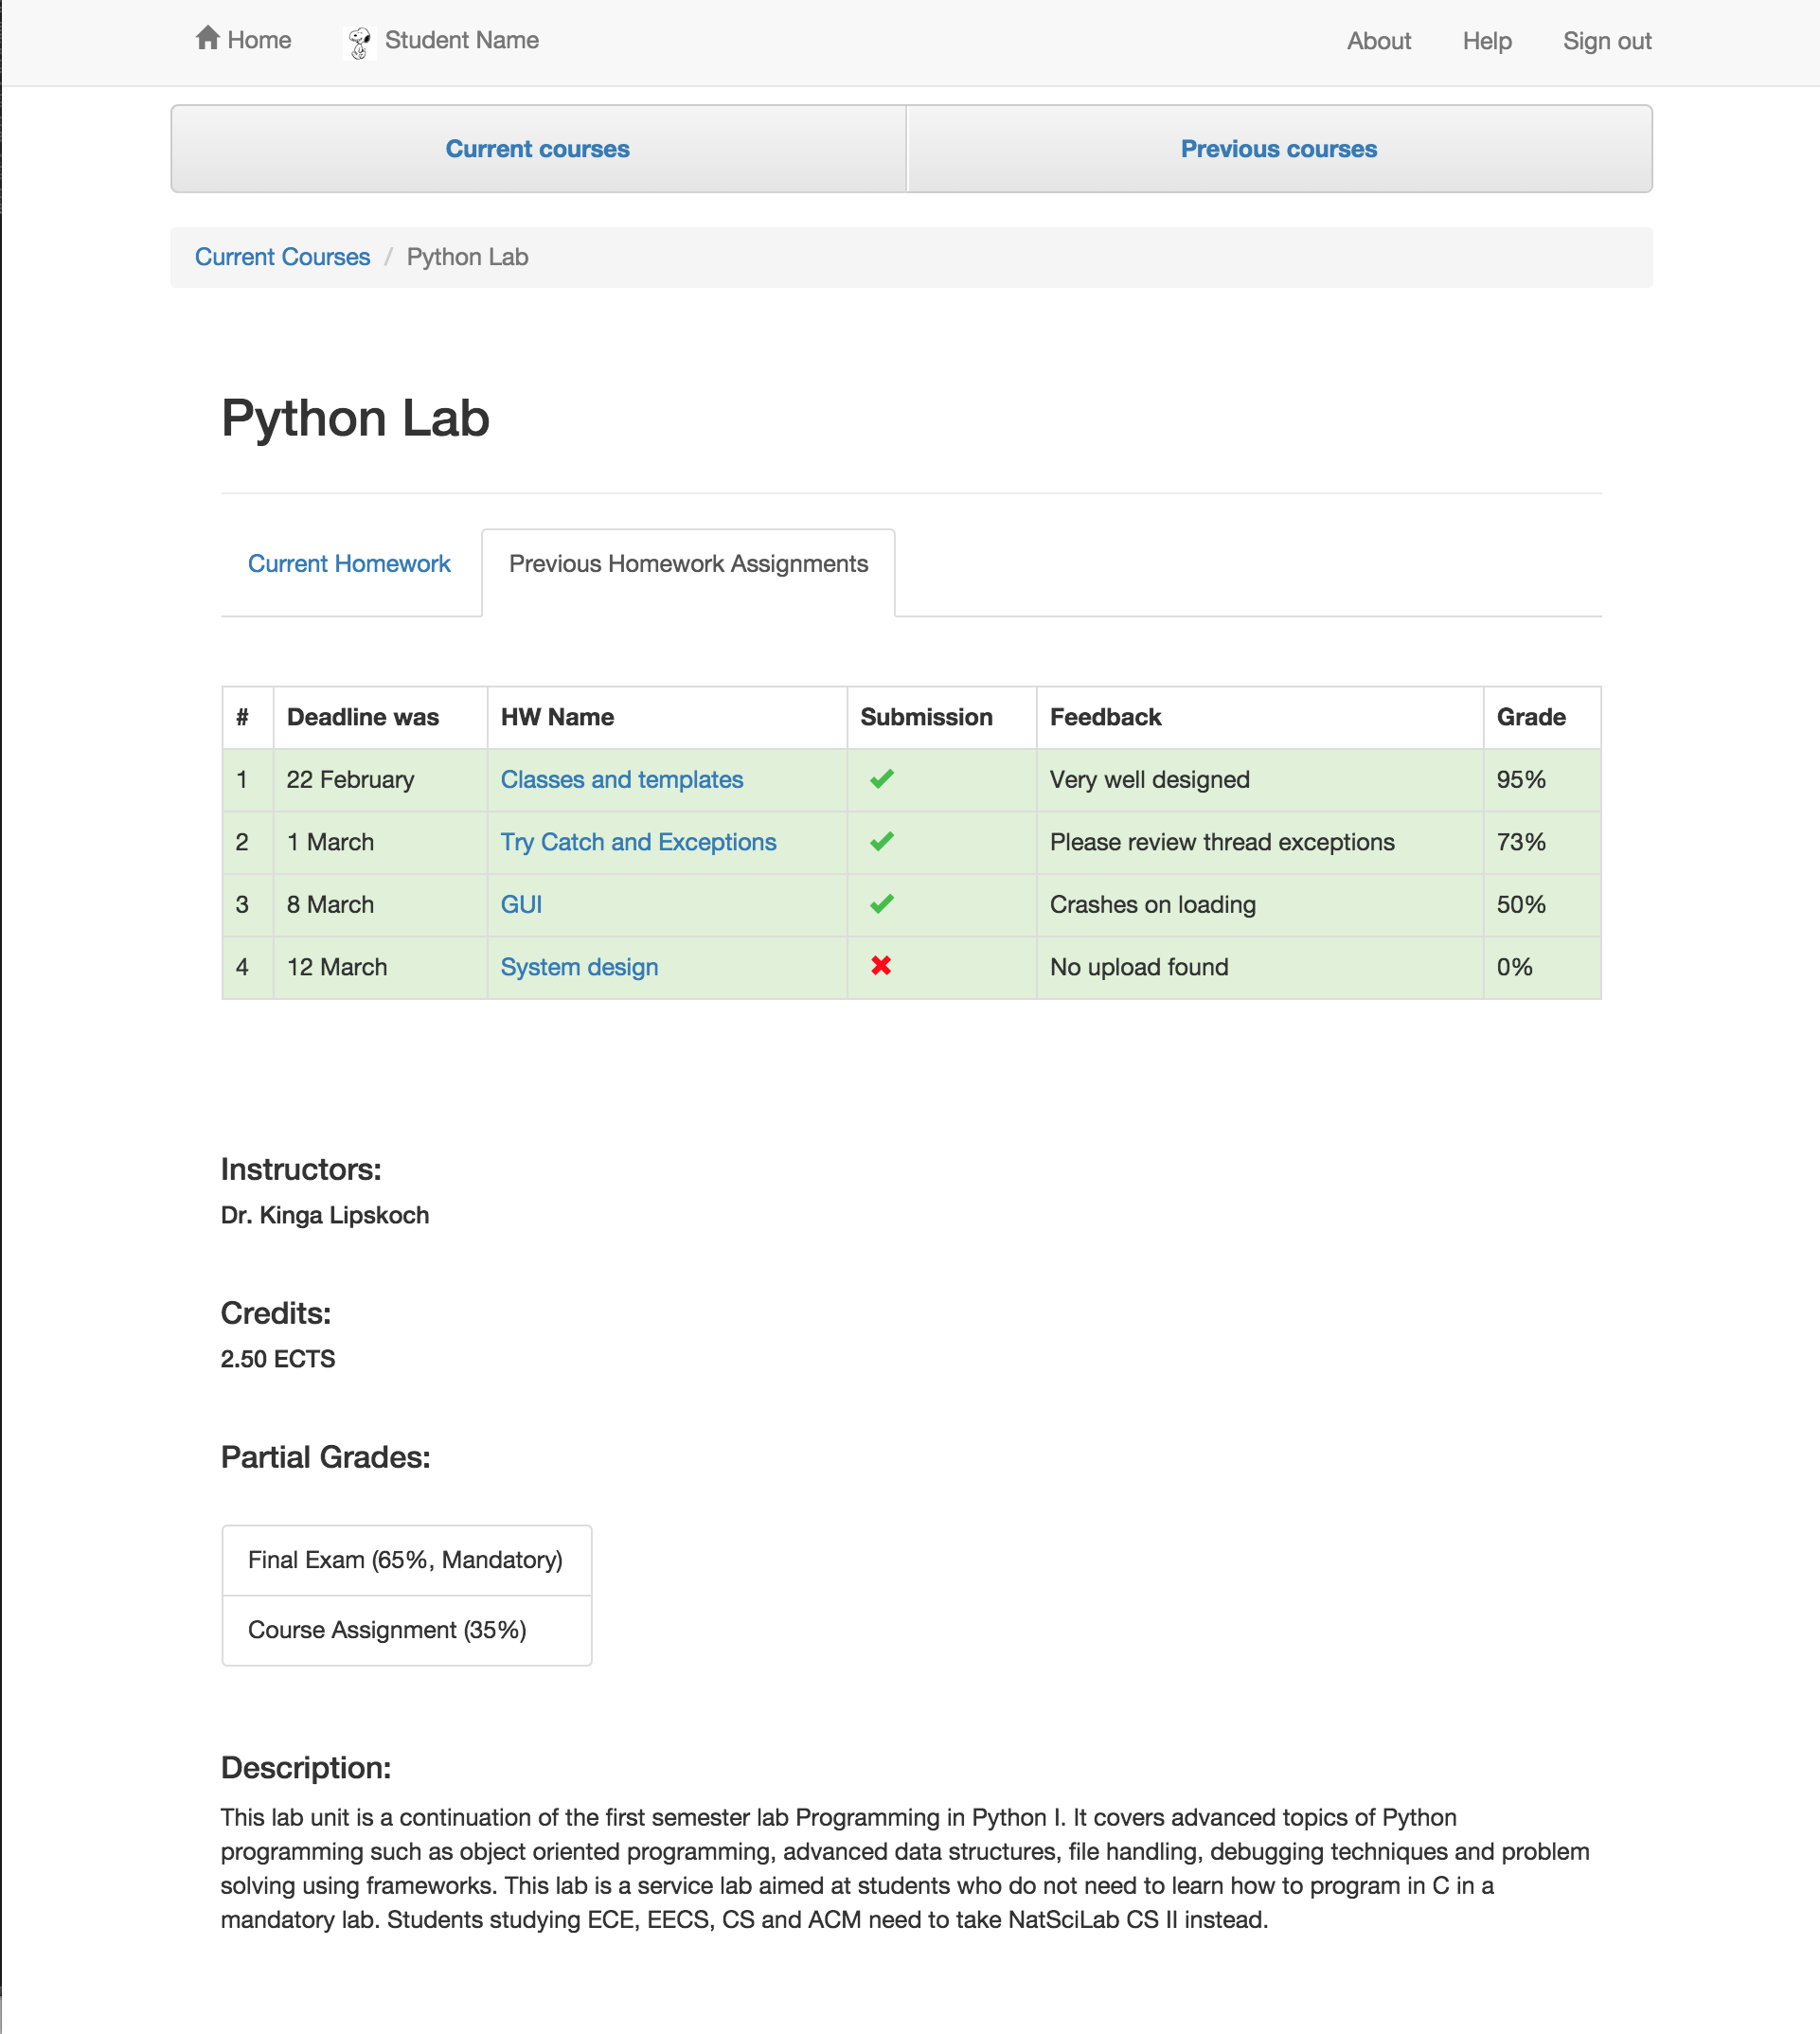
\includegraphics[width=\textwidth]{screenshots/PythonOverview.png}\newpage
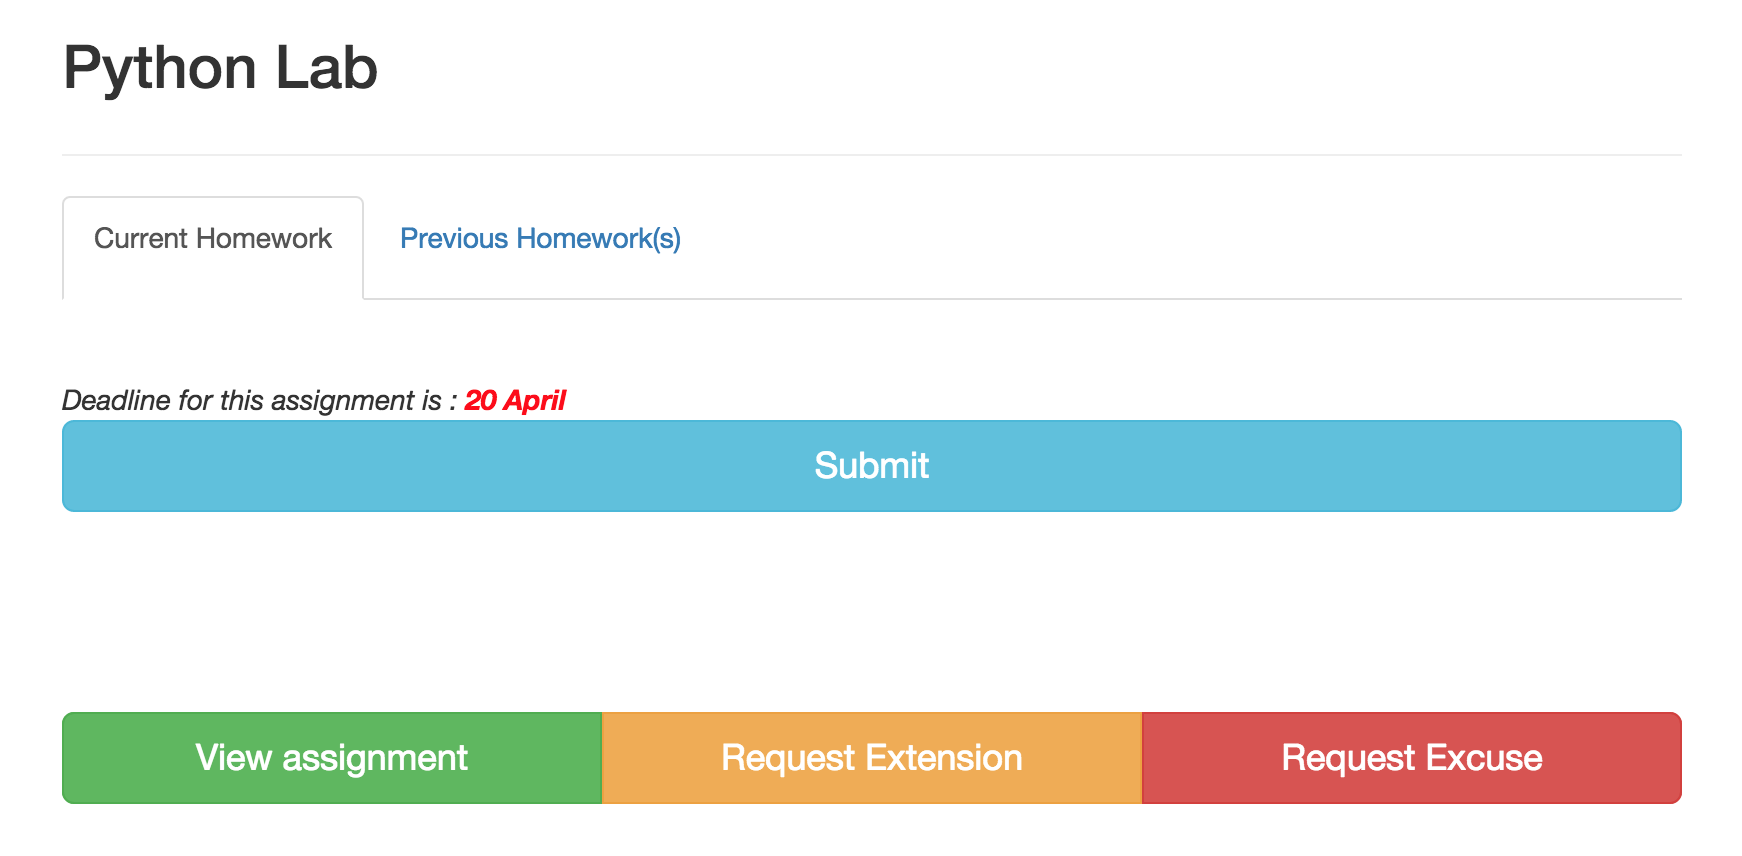
\includegraphics[width=\textwidth]{screenshots/OtherPythonOverview.png}\newline

The course page layout is designed to provide an easy to use and comprehensive dashboard for each course. It contains current assignments, previous assignments, tools to view further information, request extensions \& excuses, and an overview of the course grading breakdown, instructors, credits, and other important information.

More frequently accessed elements, such as the assignment page, are located at the top of the screen to minimise scrolling. Small amounts of color are used to highlight actionable items in order to help the user quickly find what they need. In some situations, the student may only have minutes or even seconds to submit a file, and navigational aids help. A large and wide submit button means that the user only has to search vertically through the page.
